\documentclass{standalone}
\usepackage{graphicx}	
\usepackage{amssymb, amsmath}
\usepackage{color}

\usepackage{tikz}
\usetikzlibrary{intersections, backgrounds, math}
\usepackage{pgfmath}

\definecolor{light}{RGB}{220, 188, 188}
\definecolor{mid}{RGB}{185, 124, 124}
\definecolor{dark}{RGB}{143, 39, 39}
\definecolor{highlight}{RGB}{180, 31, 180}
\definecolor{light_teal}{RGB}{107, 142, 142}
\definecolor{mid_teal}{RGB}{72, 117, 117}
\definecolor{dark_teal}{RGB}{29, 79, 79}
\definecolor{gray10}{gray}{0.1}
\definecolor{gray20}{gray}{0.2}
\definecolor{gray30}{gray}{0.3}
\definecolor{gray40}{gray}{0.4}
\definecolor{gray60}{gray}{0.6}
\definecolor{gray70}{gray}{0.7}
\definecolor{gray80}{gray}{0.8}
\definecolor{gray90}{gray}{0.9}
\definecolor{gray95}{gray}{0.95}

\begin{document}

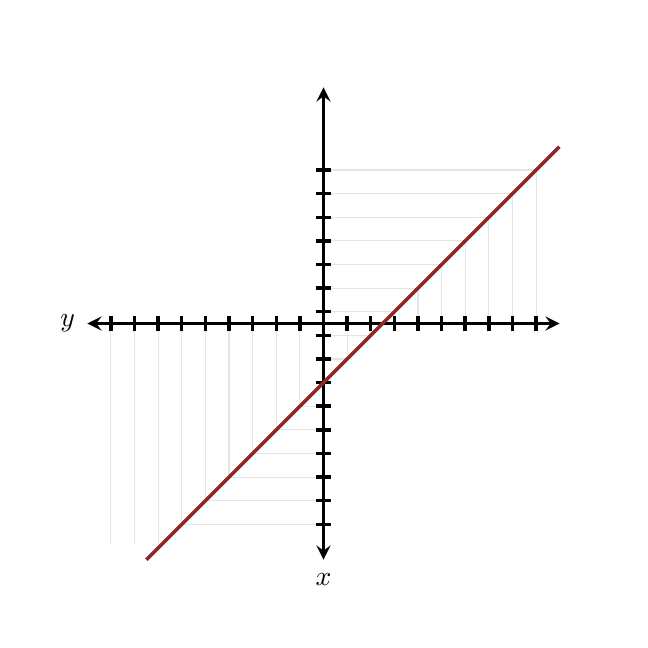
\begin{tikzpicture}[scale=1.0]

  \draw[white] (-3.75, -3.75) rectangle (3.75, 3.75);
  
  \pgfmathsetmacro{\ys}{3};
  
  \begin{scope}
    \clip (-3, -2.8) rectangle (3, 2.8);
    \foreach \x in {-0.9, -0.8, ..., 0.9} {
      \pgfmathsetmacro{\xp}{3 * \x};
      \pgfmathsetmacro{\yp}{\ys * (\x - 0.25)};
      \draw[gray90] (\xp, 0) -- (\xp, \yp) -- (0, \yp);
    }
    
    \foreach \x in {-0.9, -0.8, ..., 0.9} {
      \draw[line width=1.25] (3 * \x, -0.1) -- +(0, 0.2);
      \draw[line width=1.25] (-0.1, {\ys * (\x - 0.25)}) -- +(0.2, 0);
    }
  \end{scope}

  \draw [<->, >=stealth, line width=1.25] (0, -3) -- +(0, 6);
  \draw [<->, >=stealth, line width=1.25] (-3, 0) -- +(6, 0);
  
  \draw[domain={-0.75:1}, smooth, samples=150, line width=1.25, variable=\x, color=dark] 
    plot ({3 * \x},{\ys * (\x - 0.25)});
  
 
  \node at (-3.25, 0) { $y$ };
  \node at (0, -3.25) { $x$ };

  
\end{tikzpicture}

\end{document}  